\documentclass[12pt, a4paper]{report}

% ==============================================================================
% UPRO THESIS TEMPLATE - MAIN FILE
% ==============================================================================

% Recommended Packages
\usepackage{graphicx}       % For handling images
\usepackage{amsmath, amssymb} % For mathematical symbols
\usepackage{geometry}       % For page layout
\usepackage{setspace}       % For line spacing
\usepackage{cite}           % For IEEE citations
\usepackage{hyperref}       % For hyperlinks in PDF
\usepackage{titlesec}       % For custom chapter/section formatting
\usepackage{caption}        % For better caption formatting
\usepackage{listings}       % For code listings
\usepackage{booktabs}       % For professional table formatting
\usepackage{xcolor}         % For code highlighting
\usepackage{tikz}           % For flowcharts
\usetikzlibrary{shapes.geometric, arrows, positioning}

% TikZ Styles - Mermaid-like Theme
\tikzstyle{startstop} = [rectangle, rounded corners, minimum width=3cm, minimum height=1cm, text centered, draw=blue!60!black, fill=blue!5, thick]
\tikzstyle{process} = [rectangle, rounded corners, minimum width=3cm, minimum height=1cm, text centered, draw=blue!60!black, fill=blue!5, thick]
\tikzstyle{decision} = [diamond, aspect=2, minimum width=3cm, minimum height=1cm, text centered, draw=blue!60!black, fill=blue!5, thick]
\tikzstyle{arrow} = [thick,->,>=stealth, draw=blue!60!black]

% Code Listing Settings
\lstset{
  basicstyle=\ttfamily\small,
  breaklines=true,
  frame=single,
  keywordstyle=\color{blue},
  stringstyle=\color{red},
  commentstyle=\color{green!50!black},
  showstringspaces=false,
  numbers=left,
  numberstyle=\tiny\color{gray},
  captionpos=b
}

% Page Layout Settings (UPRO Standard)
\geometry{
    top=2.5cm,
    bottom=2.5cm,
    left=3.5cm, % Binding margin
    right=2.5cm
}
\onehalfspacing % Standard 1.5 line spacing

% Hyperlink Setup
\hypersetup{
    colorlinks=true,
    linkcolor=black,
    filecolor=magenta,      
    urlcolor=blue,
    citecolor=black
}

\begin{document}

% ==============================================================================
% METADATA - TO BE FILLED
% ==============================================================================
\title{DESIGN AND SIMULATION OF AN EXPLAINABLE AI-BASED PREDICTIVE MAINTENANCE SYSTEM FOR MARINE DIESEL ENGINES}
\author{Nahadi Farid Muigu \\ Mosonik Zadock Kiprono}
\date{\today}

% ==============================================================================
% FRONT MATTER
% ==============================================================================

% Custom Title Page
\begin{titlepage}
\thispagestyle{empty}
\begin{center}

{\setstretch{1.8}

\vspace*{1cm}

\textbf{JOMO KENYATTA UNIVERSITY OF AGRICULTURE AND TECHNOLOGY}\\[0.5cm]

\begin{figure}[h]
  \centering
  \includegraphics[width=0.3\textwidth]{./media/JKUAT-LOGO.png}
\end{figure}

\vspace{0.5cm}

\textbf {School of Mechanical Manufacturing and Materials Engineering}\\
\textbf{Department of Marine Engineering Maritime Operations}\\
\textbf{Bachelor of Science in Marine Engineering}\\
\textbf{Design and Simulation of an Explainable AI-based Predictive Maintenance System for Marine Diesel Engines}\\

\textbf{By:}

MOSONIK Zadock Kiprono : ENM241-0139/2021  \\
NAHADI Farid Muigu  : ENM241-0143/2021  \\


\vspace{0.5cm}

\textbf{SUPERVISOR}\\[0.3cm]
Dr. CHRISTIAAN Adika Adenya

\vspace{0.5cm}

A Thesis Submitted In Partial Fulfillment For The Award Of The Degree Of Bachelor Of Science In Marine Engineering}

\end{center}
\end{titlepage}

\clearpage

%----------------------------------------------------------------------------------------
%	PREAMBLE PAGES (Matches EMR 2437 Section 2.1.2)
%----------------------------------------------------------------------------------------

\pagenumbering{roman} % Roman numerals for preamble

% 1. Declaration
\section*{DECLARATION}
\addcontentsline{toc}{section}{Declaration}

We hereby declare that this thesis is our original work and has not been presented for a degree in any other university or for any other award.

\vspace{1cm}
\noindent
\textbf{Name:} MOSONIK Zadock Kiprono \hfill \textbf{REG NUMBER:} ENM241-0139/2021\\
\vspace{0.5cm}

\noindent
\textbf{Signature:} \underline{\hspace{5cm}} \hfill \textbf{Date:} \underline{\hspace{4cm}} \\

\vspace{1cm}
\noindent
\textbf{Name:} NAHADI Farid Muigu \hfill \textbf{REG NUMBER:} ENM241-0143/2021\\
\vspace{0.5cm}

\noindent
\textbf{Signature:} \underline{\hspace{5cm}} \hfill \textbf{Date:} \underline{\hspace{4cm}} \\

\vspace{1cm}
\noindent
\textbf{Supervisor Declaration:} \\

\noindent
This thesis has been submitted for examination with my approval as the University Supervisor.

\vspace{1cm}

\noindent
\textbf{Name:} Dr. CHRISTIAAN Adika Adenya
\vspace{1cm}

\noindent
\textbf{Signature:} \underline{\hspace{5cm}} \hfill \textbf{Date:} \underline{\hspace{4cm}} \\

\newpage

% 2. List of Abbreviations and Symbols
\section*{LIST OF ABBREVIATIONS AND SYMBOLS}
\addcontentsline{toc}{section}{List of Abbreviations and Symbols}

\subsection*{Abbreviations}
\begin{tabular}{ll}
\textbf{AI} & Artificial Intelligence \\
\textbf{API} & Application Programming Interface \\
\textbf{GBDT} & Gradient Boosting Decision Trees \\
\textbf{GOSS} & Gradient-based One-Side Sampling \\
\textbf{LightGBM} & Light Gradient Boosting Machine \\
\textbf{ML} & Machine Learning \\
\textbf{PdM} & Predictive Maintenance \\
\textbf{RBF} & Radial Basis Function \\
\textbf{RPM} & Revolutions Per Minute \\
\textbf{SHAP} & SHapley Additive exPlanations \\
\textbf{SMOTE} & Synthetic Minority Over-sampling Technique \\
\textbf{SVM} & Support Vector Machine \\
\textbf{TPE} & Tree-structured Parzen Estimator \\
\textbf{XAI} & Explainable Artificial Intelligence \\
\textbf{XPM} & Explainable Predictive Maintenance \\
\end{tabular}

\vspace{1cm}

\subsection*{Symbols}
\begin{tabular}{ll}
$C_0$ & Normal Operation (Fault Class 0) \\
$C_1$ & Fuel Injection Fault (Fault Class 1) \\
$C_2$ & Cooling System Fault (Fault Class 2) \\
$C_3$ & Turbocharger Fault (Fault Class 3) \\
$C_4$ & Bearing Wear (Fault Class 4) \\
$C_5$ & Lubrication Oil Degradation (Fault Class 5) \\
$C_6$ & Air Intake Blockage (Fault Class 6) \\
$C_7$ & Vibration Anomaly (Fault Class 7) \\
$\eta$ & Learning Rate \\
$\lambda$ & Random interpolation factor (SMOTE) \\
$\mu_{train}$ & Mean of training set features \\
$\sigma_{train}$ & Standard deviation of training set features \\
$\phi_i$ & SHAP value for feature $i$ \\
$F_m(x)$ & Ensemble prediction after $m$ trees \\
$h_m(x)$ & Prediction of the $m$-th tree \\
$L(p)$ & Loss function for partition $p$ \\
$M$ & Total number of features \\
$P_{air}$ & Air Pressure (bar) \\
$P_{cyl}$ & Cylinder Pressure (bar) \\
$P_{oil}$ & Oil Pressure (bar) \\
$T_{exh}$ & Exhaust Temperature (°C) \\
$Vib_x$ & Vibration X-axis (mm/s) \\
$Vib_y$ & Vibration Y-axis (mm/s) \\
$Vib_z$ & Vibration Z-axis (mm/s) \\
$z$ & Normalized feature value (Z-score) \\
\end{tabular}

\newpage

\chapter*{Abstract}
\addcontentsline{toc}{chapter}{Abstract}
Metric-driven maintenance strategies are evolving towards predictive approaches to enhance reliability and safety in the maritime industry. This thesis presents the design and simulation of an Explainable AI (XAI)-based predictive maintenance system for marine diesel engines. Using a synthetic dataset of 10,000 operational samples from a 4-cylinder engine, a Light Gradient Boosting Machine (LightGBM) model was developed to classify 8 distinct engine states, including cooling, lubrication, and turbocharger faults. The model achieved a Macro F1-Score of 0.80, demonstrating exceptional performance on mechanical faults (100\% F1 for Bearing Wear) while revealing challenges in detecting subtle thermodynamic anomalies (30\% F1 for Fuel Injection). To address the opacity of machine learning models, SHapley Additive exPlanations (SHAP) were integrated, enabling transparent root-cause analysis by quantifying the contribution of individual sensors to each diagnosis. A full-stack prototype, featuring a FastAPI backend and React.js dashboard, was deployed to demonstrate real-time inference capabilities ($<$2ms latency) suitable for edge computing on vessels. The findings indicate that while the system excels at detecting critical mechanical failures, future work should explore ensemble methods to improve thermodynamic fault classification.

\chapter*{Acknowledgements}
\addcontentsline{toc}{chapter}{Acknowledgements}

We would like to express our sincere gratitude to all those who contributed to the successful completion of this thesis.

First and foremost, we extend our deepest appreciation to our supervisor, \textbf{Dr. CHRISTIAAN Adika Adenya}, for his invaluable guidance, constructive feedback, and unwavering support throughout this research project. His expertise in marine engineering and commitment to academic excellence have been instrumental in shaping this work.

Our sincere thanks go to all the lecturers and staff members who have imparted knowledge and skills throughout our undergraduate studies, laying the foundation for this research endeavor.

We acknowledge the open-source community for developing and maintaining the machine learning libraries (LightGBM, SHAP, Scikit-learn) and web development frameworks (FastAPI, React.js) that made this project possible.

Finally, we thank the Almighty God for granting us the health, wisdom, and perseverance to complete this thesis.

\tableofcontents
\listoffigures
\listoftables
\newpage

% ==============================================================================
% MAIN CONTENT
% ==============================================================================
% Arabic numerals for main content
\pagenumbering{arabic}
% Chapters will be included here

\chapter{Introduction}
\label{chap:introduction}

\section{Background}
Marine diesel engines form the backbone of the global maritime industry, powering over 90\% of commercial vessels responsible for transporting global trade. The reliability of these engines is paramount; any failure can lead to severe operational disruptions, financial losses, and safety hazards. Traditional maintenance strategies, such as corrective (run-to-failure) and preventive (schedule-based) maintenance, often prove inefficient or costly. Corrective maintenance results in unpredictable downtime, while preventive maintenance can lead to unnecessary replacement of healthy components.

\section{Problem Statement}
Current engine monitoring systems largely rely on static threshold alarms. These systems trigger alerts only when a parameter exceeds a pre-defined limit. This approach has significant limitations:
\begin{enumerate}
    \item \textbf{High False Positive Rate:} Transient operational changes can trigger false alarms.
    \item \textbf{Lack of Prognostics:} Alarms occur after degradation has reached a critical level, offering little time for proactive intervention.
    \item \textbf{No Root Cause Analysis:} A generic ``high temperature'' alarm does not specify whether the cause is a cooling system failure, lubrication issue, or bearing wear.
\end{enumerate}
There is a critical need for a system that can not only predict faults before they occur but also explain the reasoning behind its predictions to engine operators.

\section{Objectives}
The primary objective of this project is to design and simulate an Explainable AI (XAI) based predictive maintenance system for marine diesel engines. Specific objectives include:
\begin{enumerate}
    \item To simulate a realistic dataset for a 4-cylinder marine diesel engine covering normal operation and eight specific fault conditions.
    \item To design a predictive model using the Light Gradient Boosting Machine (LightGBM) algorithm to classify engine health states.
    \item To implement SHAP (SHapley Additive exPlanations) to provide interpretable explanations for model predictions, identifying key contributing sensors.
    \item To develop a real-time engineering dashboard using React and FastAPI to visualize engine health and diagnostic insights.
\end{enumerate}

\section{Significance}
This research contributes to the maritime industry's transition towards ``Intelligent Vessels.'' By moving from reactive to predictive maintenance, ship operators can:
\begin{itemize}
    \item Reduce operational expenditure (OPEX) by optimizing maintenance schedules.
    \item Enhance safety by preventing catastrophic engine failures at sea.
    \item improve decision-making confidence through transparent, explainable AI diagnostics.
\end{itemize}

\section{Scope}
The scope of this project is limited to:
\begin{itemize}
    \item \textbf{Target System:} A simulated 4-cylinder marine diesel engine.
    \item \textbf{Fault Classes:} Normal operation and seven fault types including Fuel Injection Fault, Cooling System Fault, Turbocharger Fault, Bearing Wear, Lubrication Oil Degradation, Air Intake Restriction, and Vibration Anomaly.
    \item \textbf{Data:} Synthetic data generated to mimic real-world sensor behavior (18 parameters).
    \item \textbf{Verification:} Validation is performed via simulation scenarios; physical engine testing is outside the scope.
\end{itemize}

\chapter{Literature Review}
\label{chap:literature_review}

\section{Introduction}
The maritime industry stands on the precipice of a digital transformation, moving from traditional reactive maintenance to intelligent, data-driven strategies. This chapter provides a critical analysis of the current state of predictive maintenance (PdM) for marine diesel engines, evaluating the strengths and limitations of contemporary Machine Learning (ML) algorithms and the emerging necessity for Explainable AI (XAI) to ensure trustworthiness in autonomous systems.

\section{Evolution of Maintenance Strategies in Maritime}
Historically, marine machinery maintenance has followed a "Run-to-Failure" (Corrective) or "Time-Based" (Preventive) approach. \cite{marine_engine_maintenance} notes that while preventive maintenance reduces catastrophic failures, it often leads to the premature replacement of healthy components, inflating Operational Expenditure (OPEX). 

Condition-Based Maintenance (CBM), and subsequently Predictive Maintenance (PdM), offer a solution by utilizing real-time sensor data to forecast equipment health. A framework proposed by \cite{ml_framework_marine_2024} demonstrates that integrating IoT sensors with predictive analytics can extend engine useful life by up to 15\% and reduce downtime by 30\%. However, the implementation of such systems faces significant hurdles. \cite{maritime_data_challenges} highlights that data heterogeneity and intermittent satellite connectivity remain primary bottlenecks, often following the "Garbage In, Garbage Out" principle where poor sensor quality leads to unreliable predictions.

\section{Comparative Analysis of Machine Learning Algorithms}
The core of any PdM system is the diagnostic algorithm. Recent literature has extensively compared various approaches for marine engine fault detection.

\subsection{Support Vector Machines (SVM) vs. Random Forest (RF)}
SVMs have long been favored for their robustness in high-dimensional spaces. \cite{svm_vs_rf_marine} found SVMs to be highly effective for binary classification of specific faults but noted their scalability issues with large, continuous sensor streams. In contrast, Random Forest (RF) ensembles offer better generalizability and resistance to overfitting. However, \cite{pdm_diesel_gen_2025} argues that RF models can become computationally heavy for edge deployment on vessels with limited hardware resources.

\subsection{The Rise of LightGBM}
Light Gradient Boosting Machine (LightGBM), introduced by \cite{ke2017lightgbm}, represents the state-of-the-art in gradient boosting frameworks. It utilizes a leaf-wise tree growth strategy and histogram-based algorithms, offering significant advantages over SVM and RF:
\begin{enumerate}
    \item \textbf{Training Speed:} LightGBM fits 10-20x faster than traditional Gradient Boosting Decision Trees (GBDT).
    \item \textbf{Accuracy:} It consistently achieves higher classification accuracy in tabular sensor data.
    \item \textbf{Memory Efficiency:} Its bucket-based logic reduces memory consumption, making it ideal for the constrained computing environments found on ships.
\end{enumerate}
Despite these advantages, gradient boosting models are inherently "black boxes," lacking the transparency required for critical safety systems.

\section{Explainable AI (XAI): Bridging the Trust Gap}
As AI systems become more complex, their decision-making opacity becomes a liability. In safety-critical marine environments, an operator cannot trust a "Check Engine" alert without understanding the underlying cause. \cite{survey_xpm_2024} defines Explainable Predictive Maintenance (XPM) as the integration of interpretability techniques into diagnostic workflows.

\subsection{LIME vs. SHAP}
Two dominant post-hoc explanation methods were evaluated by \cite{shap_vs_lime_pdm}:
\begin{itemize}
    \item \textbf{LIME (Local Interpretable Model-agnostic Explanations):} Perturbs local inputs to approximate linear explanations. While fast, it suffers from instability where similar inputs can yield different explanations.
    \item \textbf{SHAP (SHapley Additive exPlanations):} Proposed by \cite{lundberg2017unified}, SHAP is grounded in cooperative game theory. It guarantees consistency and local accuracy, ensuring that the sum of feature contributions equals the model's prediction deviation.
\end{itemize}
\cite{framework_lstm_xai_2024} successfully applied SHAP to LSTM models for main engines, proving that SHAP provides more reliable engineering insights (e.g., identifying that "High Exhaust Temp" + "Low RPM" = "Injector Fault") compared to LIME.

\section{Research Gaps and Proposed Contribution}
While the literature establishes the efficacy of LightGBM and the necessity of XAI, few studies combine them specifically for 4-cylinder marine diesel engines using a comprehensive sensor suite. Existing frameworks often focus on auxiliary generators \cite{pdm_diesel_gen_2025} or utilize computationally expensive Deep Learning models \cite{framework_lstm_xai_2024}.

This thesis bridges this gap by designing a system that:
\begin{enumerate}
    \item Leverages the speed and accuracy of \textbf{LightGBM} for real-time classification.
    \item Integrates \textbf{SHAP} values to distinctively diagnose 8 specific fault classes (Scope Match).
    \item Addresses the \textbf{data imbalance} challenge using SMOTE, a critical preprocessing step often overlooked in general maritime surveys.
\end{enumerate}
By validating this approach on a simulated 18-parameter dataset, this research contributes a verified, explainable framework for modern smart vessels.

\chapter{Methodology}
\label{chap:methodology}

\section{Introduction}
This chapter delineates the engineering framework designed to develop the Explainable Predictive Maintenance (XPM) system. The methodology follows a rigorous data science usage lifecycle, tailored specifically for the distinctive thermodynamic characteristics of marine propulsion. It encompasses data acquisition, advanced preprocessing using synthetic oversampling, model development via gradient boosting, and the integration of game-theoretic explainability. Figure \ref{fig:methodology_flow} illustrates the high-level architecture.

\begin{figure}[h]
    \centering
    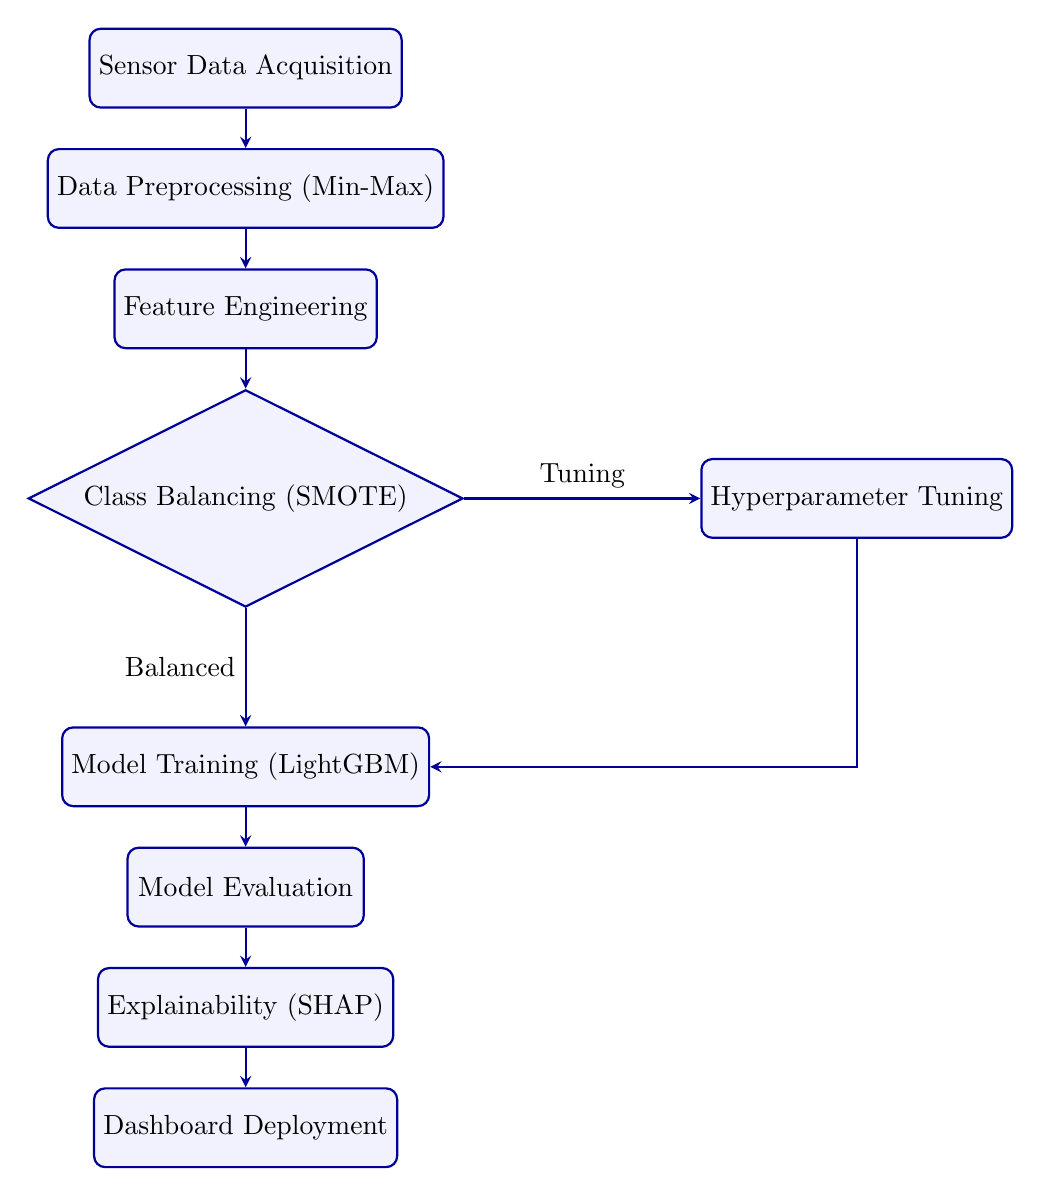
\begin{tikzpicture}[node distance=0.5cm]
        % Nodes
        \node (start) [startstop] {Sensor Data Acquisition};
        \node (pro1) [process, below=of start] {Data Preprocessing (Min-Max)};
        \node (pro2) [process, below=of pro1] {Feature Engineering};
        \node (dec) [decision, below=of pro2] {Class Balancing (SMOTE)};
        
        % Split paths for decision
        \node (pro3) [process, below=of dec, yshift=-1.0cm] {Model Training (LightGBM)};
        \node (opt) [process, right=of dec, xshift=2.5cm] {Hyperparameter Tuning};
        
        \node (eval) [process, below=of pro3] {Model Evaluation};
        \node (xai) [process, below=of eval] {Explainability (SHAP)};
        \node (end) [startstop, below=of xai] {Dashboard Deployment};

        % Arrows
        \draw [arrow] (start) -- (pro1);
        \draw [arrow] (pro1) -- (pro2);
        \draw [arrow] (pro2) -- (dec);
        
        % SMOTE loop
        \draw [arrow] (dec) -- node[anchor=east] {Balanced} (pro3);
        \draw [arrow] (dec) -- node[anchor=south] {Tuning} (opt);
        \draw [arrow] (opt) |- (pro3);
        
        \draw [arrow] (pro3) -- (eval);
        \draw [arrow] (eval) -- (xai);
        \draw [arrow] (xai) -- (end);
    \end{tikzpicture}
    \caption{Proposed XPM Methodology Workflow}
    \label{fig:methodology_flow}
\end{figure}

\section{Data Acquisition and Marine Engineering Context}
The research utilizes a high-fidelity synthetic dataset representative of a **Medium-Speed 4-Stroke Marine Diesel Engine** (operating range 800-1200 RPM). This engine class is ubiquitous in maritime auxiliary power generation and coastal propulsion.

\subsection{Thermodynamic Cycle and Fault Correlation}
The monitored parameters are not merely statistical features but direct indicators of the Diesel operational cycle. 
\begin{enumerate}
    \item \textbf{Combustion Health (Exhaust Temperatures):} In a 4-stroke cycle, deviation in exhaust gas temperature ($T_{exh}$) is the primary indicator of combustion efficiency.
    \begin{itemize}
        \item \textit{High $T_{exh}$:} Indicates "after-burning" typically caused by late injection timing or leaky exhaust valves.
        \item \textit{Low $T_{exh}$ + White Smoke:} Correlates with water ingress (Cooling Fault) or incomplete combustion due to low compression.
    \end{itemize}
    \item \textbf{Mechanical Integrity (Vibration):} The 4-stroke cycle introduces specific vibration orders ($0.5 \times RPM$, $1 \times RPM$). Elevated lateral (X-axis) vibration often signals piston slap or crosshead wear, while axial (Z-axis) vibration points to thrust bearing degradation.
    \item \textbf{Scavenging Efficiency (Air Pressure):} Turbocharger performance is critical. A drop in manifold air pressure ($P_{air}$) directly results in a rich fuel mixture, leading to high thermal stress and potential "Black Smoke" emissions.
\end{enumerate}

\subsection{Feature Space Definition}
The 18-parameter feature space (Table \ref{tab:feature_space}) captures these physical phenomena.

\begin{table}[h]
    \centering
    \begin{tabular}{lll}
    \toprule
    \textbf{Category} & \textbf{Sensors} & \textbf{Unit} \\ \midrule
    Mechanical & Shaft RPM, Vibration (X, Y, Z) & RPM, mm/s \\
    Thermodynamic & Exhaust Temp (Cyl 1-4), Oil Temp & $^\circ$C \\
    Pressure & Air Pressure, Oil Pressure, Cyl Pressure (1-4) & Bar \\
    Performance & Engine Load, Fuel Flow & \%, L/hr \\ \bottomrule
    \end{tabular}
    \caption{Monitored Engine Parameters}
    \label{tab:feature_space}
\end{table}

\section{Advanced Preprocessing}
\subsection{Data Splitting}
To ensure rigorous evaluation and prevent \textit{data leakage} (where information from the test set inadvertently influences the training process), the dataset is split into training (80\%) and testing (20\%) sets using a \textbf{stratified sampling strategy}. 

\textbf{What is Stratified Sampling?} In a standard random split, minority classes (e.g., Bearing Wear at 4.8\% of the dataset) might be underrepresented or even absent in one of the subsets. Stratified sampling ensures that the proportion of each fault class remains consistent across both training and test sets. For example, if Bearing Wear constitutes 4.8\% of the full dataset, it will also constitute approximately 4.8\% of both the training and test sets.

\textbf{Why 80/20?} This ratio is a standard practice in machine learning that balances two competing needs:
\begin{itemize}
    \item \textbf{Training Set (80\%):} Provides sufficient data for the model to learn complex patterns and relationships between sensor readings and fault types.
    \item \textbf{Test Set (20\%):} Reserves enough unseen data to reliably evaluate the model's generalization performance on new, real-world scenarios.
\end{itemize}

\subsection{Normalization (Feature Scaling)}
\textbf{The Problem:} Marine engine sensors measure vastly different physical quantities with incompatible scales:
\begin{itemize}
    \item Cylinder Pressure: $\approx$ 140 bar (large magnitude)
    \item Vibration X-axis: $\approx$ 0.1 mm/s (small magnitude)
    \item Shaft RPM: $\approx$ 1000 RPM (medium magnitude)
\end{itemize}

Without normalization, machine learning algorithms would treat features with larger numerical ranges as more important, even if they're less relevant for fault detection. For instance, a 1-unit change in cylinder pressure (140 → 141 bar) would be weighted 1400 times more heavily than a 1-unit change in vibration (0.1 → 1.1 mm/s), despite vibration being a critical fault indicator.

\textbf{Solution: Standard Scaling (Z-score Normalization)}

We apply the following transformation to each feature:
\begin{equation}
    z = \frac{x - \mu_{train}}{\sigma_{train}}
\end{equation}

\textbf{Breaking Down the Equation:}
\begin{itemize}
    \item $x$: The original sensor value (e.g., 142 bar for cylinder pressure)
    \item $\mu_{train}$: The \textit{mean} (average) of that sensor's values in the training set
    \item $\sigma_{train}$: The \textit{standard deviation} (measure of spread) of that sensor's values in the training set
    \item $z$: The normalized value (typically between -3 and +3)
\end{itemize}

\textbf{Example Calculation:}
Suppose for Oil Pressure in the training set:
\begin{itemize}
    \item Mean ($\mu_{train}$) = 3.5 bar
    \item Standard Deviation ($\sigma_{train}$) = 0.5 bar
    \item New test sample: $x = 4.0$ bar
\end{itemize}
Then: $z = \frac{4.0 - 3.5}{0.5} = \frac{0.5}{0.5} = 1.0$

This means the oil pressure is 1 standard deviation above the training average—a standardized measure that can be compared across all sensors.

\textbf{Critical Implementation Detail:} The scaler is fit \textit{only} on the training set ($\mu_{train}$, $\sigma_{train}$) and then applied to the test set. This mimics real-world deployment where future data statistics are unknown. If we calculated $\mu$ and $\sigma$ on the test set, we would be "peeking" at future data, leading to overly optimistic performance estimates.

\subsection{Synthetic Minority Over-sampling Technique (SMOTE)}
\textbf{The Class Imbalance Problem:}
In maritime operations, engines spend most of their time in healthy states. Our dataset reflects this reality:
\begin{itemize}
    \item Normal Operation ($C_0$): 60\% of samples
    \item Bearing Wear ($C_4$): 4.8\% of samples
    \item Fuel Injection Fault ($C_1$): 5.2\% of samples
\end{itemize}

This creates a "Normalcy Bias" where the model learns to predict "Normal" most of the time, achieving high overall accuracy (e.g., 60\%) while completely failing to detect critical faults.

\textbf{SMOTE Algorithm Explained:}
SMOTE (Synthetic Minority Over-sampling Technique) addresses this by creating \textit{synthetic} (artificial but realistic) samples of minority classes. It does NOT simply duplicate existing fault samples (which would lead to overfitting), but instead generates new, plausible fault scenarios.

\textbf{How SMOTE Works (Step-by-Step):}
\begin{enumerate}
    \item \textbf{Select a minority sample:} Choose a random sample $x_i$ from a minority class (e.g., a Bearing Wear instance).
    \item \textbf{Find nearest neighbors:} Identify the $k$ nearest neighbors of $x_i$ within the same class (typically $k=5$). "Nearest" is measured using Euclidean distance in the feature space.
    \item \textbf{Choose a neighbor:} Randomly select one of these neighbors, call it $x_{zi}$.
    \item \textbf{Generate synthetic sample:} Create a new sample $x_{new}$ by interpolating between $x_i$ and $x_{zi}$:
\end{enumerate}

\begin{equation}
    x_{new} = x_i + \lambda \times (x_{zi} - x_i)
\end{equation}

\textbf{Understanding the Equation:}
\begin{itemize}
    \item $x_i$: The original minority sample (e.g., a Bearing Wear instance with specific sensor readings)
    \item $x_{zi}$: A nearby sample from the same class
    \item $\lambda$: A random number between 0 and 1 (e.g., 0.3, 0.7, 0.5)
    \item $(x_{zi} - x_i)$: The "direction vector" from $x_i$ to $x_{zi}$
    \item $\lambda \times (x_{zi} - x_i)$: A fraction of that direction (e.g., 30\% of the way from $x_i$ to $x_{zi}$)
    \item $x_{new}$: The new synthetic sample, positioned somewhere along the line connecting $x_i$ and $x_{zi}$
\end{itemize}

\textbf{Geometric Interpretation:} If you imagine the feature space as a map, SMOTE draws a line between two similar fault instances and places a new synthetic instance somewhere along that line. This expands the "decision boundary" (the region the model associates with that fault) without simply copying existing data.

\textbf{Example:}
Suppose we have two Bearing Wear samples:
\begin{itemize}
    \item $x_i$: Vibration Z = 2.5 mm/s, Oil Temp = 85°C
    \item $x_{zi}$: Vibration Z = 3.0 mm/s, Oil Temp = 90°C
    \item Random $\lambda = 0.4$
\end{itemize}

Then:
\begin{align*}
x_{new}(\text{Vibration Z}) &= 2.5 + 0.4 \times (3.0 - 2.5) = 2.5 + 0.2 = 2.7 \text{ mm/s} \\
x_{new}(\text{Oil Temp}) &= 85 + 0.4 \times (90 - 85) = 85 + 2 = 87°\text{C}
\end{align*}

This creates a realistic new Bearing Wear instance with intermediate sensor values.

\newpage
\textbf{Code Implementation:}
\begin{lstlisting}[language=Python, caption=SMOTE Implementation with Detailed Comments]
from imblearn.over_sampling import SMOTE

# Initialize SMOTE with automatic balancing strategy
# 'auto' means: balance all minority classes to match the majority class count
# random_state=42 ensures reproducibility (same synthetic samples each run)
smote = SMOTE(sampling_strategy='auto', random_state=42)

# Apply SMOTE ONLY to training data to prevent data leakage
# fit_resample() performs two operations:
#   1. fit: Learns the structure of minority classes (finds neighbors)
#   2. resample: Generates synthetic samples and returns balanced dataset
X_train_resampled, y_train_resampled = smote.fit_resample(X_train, y_train)

# After SMOTE:
# - X_train_resampled: Training features with added synthetic minority samples
# - y_train_resampled: Corresponding labels (now balanced across all classes)
# - Test set (X_test, y_test) remains unchanged (no synthetic data in evaluation)
\end{lstlisting}

\textbf{Why Only Train on Resampled Data?}
We apply SMOTE exclusively to the training set because:
\begin{enumerate}
    \item \textbf{Realistic Evaluation:} The test set should reflect real-world class imbalance. If we balanced the test set, we'd get an overly optimistic performance estimate.
    \item \textbf{No Data Leakage:} Generating synthetic test samples using training data information would contaminate the evaluation.
\end{enumerate}


\section{Model Algorithm: LightGBM}
Light Gradient Boosting Machine (LightGBM) is selected for its superior efficiency over traditional algorithms like Support Vector Machines (SVM) and Random Forests. LightGBM is an \textit{ensemble method}, meaning it combines multiple weak learners (simple decision trees) to create a strong predictive model.

\textbf{What is Gradient Boosting?}
Gradient Boosting builds trees sequentially, where each new tree attempts to correct the errors made by the previous trees. Think of it as a team of specialists where each new member focuses on the cases that the team currently struggles with. Mathematically, if we have predictions $F_{m-1}(x)$ from the first $m-1$ trees, the next tree $h_m(x)$ is trained to predict the residual error:
\begin{equation}
    F_m(x) = F_{m-1}(x) + \eta \cdot h_m(x)
\end{equation}
where $\eta$ is the learning rate (how much we trust each new tree's contribution).

\subsection{Leaf-wise Tree Growth}
\textbf{Traditional Approach (Level-wise):}
Standard Gradient Boosting Decision Trees (GBDT) grow trees level-by-level, like building a pyramid. At each level, \textit{all} nodes are split simultaneously, regardless of whether the split provides significant improvement. This is computationally wasteful.

\textbf{LightGBM's Innovation (Leaf-wise):}
LightGBM uses a "best-first" strategy, choosing to split the single leaf that will provide the maximum reduction in loss (error). This is formulated as:

\begin{equation}
    (p_L, p_R) = \arg \min_{(p_L, p_R)} \left( L(p_L) + L(p_R) \right)
\end{equation}

\textbf{Breaking Down the Equation:}
\begin{itemize}
    \item $p_L$: The left child node after splitting (e.g., samples where "Oil Pressure $<$ 3.2 bar")
    \item $p_R$: The right child node after splitting (e.g., samples where "Oil Pressure $\geq$ 3.2 bar")
    \item $L(p)$: The loss function (measure of prediction error) for partition $p$
    \item $\arg \min$: "Find the split that minimizes..." (choose the best split point)
    \item $(p_L, p_R)$: The optimal left-right partition
\end{itemize}

\textbf{Intuitive Example:}
Imagine you have a leaf containing 100 engine samples with mixed fault types. LightGBM evaluates all possible splits:
\begin{itemize}
    \item Split A: "If Vibration Z $>$ 2.0 mm/s" → Reduces loss by 15 units
    \item Split B: "If Oil Pressure $<$ 3.5 bar" → Reduces loss by 8 units
    \item Split C: "If RPM $>$ 1050" → Reduces loss by 2 units
\end{itemize}

LightGBM chooses Split A because it provides the maximum loss reduction (15 units). This strategy drastically reduces training time while achieving lower overall loss for the same number of terminal nodes.

\textbf{Advantage:} For our marine engine dataset with 18 features and 8 fault classes, leaf-wise growth focuses computational resources on the most informative splits (e.g., distinguishing Bearing Wear from Normal based on vibration), rather than wasting time on uninformative splits (e.g., splitting based on Engine Load, which is similar across fault types).

\subsection{Hyperparameter Optimization}
The model hyperparameters were optimized using \textbf{Optuna}, an automated hyperparameter tuning framework that employs a Tree-structured Parzen Estimator (TPE) to intelligently search the configuration space. After 50 trials targeting the maximization of the Macro F1-Score (our primary evaluation metric), the optimal parameters were identified as:

\begin{itemize}
    \item \textbf{Number of Estimators (n\_estimators = 323):} 
    \begin{itemize}
        \item \textit{What it means:} The total number of decision trees in the ensemble.
        \item \textit{Why 323?} More trees generally improve performance, but with diminishing returns. Optuna found that 323 trees provide the best balance between accuracy and training time. Beyond this, additional trees provide minimal improvement.
        \item \textit{Analogy:} Like having 323 expert mechanics each examining the engine from a different angle.
    \end{itemize}
    
    \item \textbf{Learning Rate ($\eta$ = 0.0685):}
    \begin{itemize}
        \item \textit{What it means:} Controls how much each tree contributes to the final prediction (see Equation 3.3).
        \item \textit{Why 0.0685?} A smaller learning rate (closer to 0) makes the model learn more slowly but more accurately. 0.0685 is relatively small, meaning each tree makes a modest contribution, requiring more trees (323) to reach optimal performance.
        \item \textit{Trade-off:} Low learning rate + many trees = better generalization but longer training time.
    \end{itemize}
    
    \item \textbf{Num Leaves (num\_leaves = 90):}
    \begin{itemize}
        \item \textit{What it means:} Maximum number of terminal nodes (leaves) in each tree.
        \item \textit{Why 90?} More leaves allow the tree to capture more complex patterns. With 90 leaves, each tree can create up to 90 distinct "rules" for classifying faults.
        \item \textit{Example:} A tree might have leaves like: "If Vibration Z $>$ 2.5 AND Oil Temp $>$ 85°C → Bearing Wear"
    \end{itemize}
    
    \item \textbf{Max Depth (max\_depth = 5):}
    \begin{itemize}
        \item \textit{What it means:} Maximum number of splits from root to leaf (tree height).
        \item \textit{Why 5?} Limits tree complexity to prevent overfitting. A depth of 5 means at most 5 sequential "if-then" decisions.
        \item \textit{Constraint:} Works with num\_leaves to control model complexity. Even with 90 allowed leaves, depth is capped at 5 levels.
    \end{itemize}
    
    \item \textbf{Subsample (subsample = 0.8137):}
    \begin{itemize}
        \item \textit{What it means:} Fraction of training samples used to build each tree.
        \item \textit{Why 0.8137?} Each tree is trained on a random 81.37\% of the data. This introduces diversity among trees (different trees see slightly different data), improving generalization.
        \item \textit{Benefit:} Reduces overfitting and speeds up training (smaller dataset per tree).
    \end{itemize}
\end{itemize}

\textbf{How Optuna Found These Values:}
Optuna uses Bayesian optimization to intelligently explore the hyperparameter space. Instead of trying random combinations, it learns from previous trials. For example, if trials with high learning rates performed poorly, Optuna focuses subsequent trials on lower learning rates. After 50 trials, it converged on the configuration above, which achieved the highest Macro F1-Score (0.80) on the validation set.

\subsection{Gradient-based One-Side Sampling (GOSS)}
To further accelerate training, LightGBM employs GOSS, a novel sampling technique that prioritizes informative instances.

\textbf{The Problem:} In traditional gradient boosting, all training samples are used to compute each split, which is computationally expensive for large datasets.

\textbf{GOSS Solution:} GOSS recognizes that not all samples are equally informative:
\begin{itemize}
    \item \textbf{Large gradient samples:} Instances with large prediction errors (e.g., a Bearing Wear case misclassified as Normal). These are \textit{highly informative} and should be retained.
    \item \textbf{Small gradient samples:} Instances already well-predicted (e.g., a Normal case correctly classified). These are \textit{less informative} and can be downsampled.
\end{itemize}

\textbf{GOSS Algorithm:}
\begin{enumerate}
    \item Sort all samples by the absolute value of their gradients (prediction errors).
    \item Keep the top $a\%$ samples with the largest gradients (set $A$).
    \item Randomly sample $b\%$ of the remaining samples (set $B$).
    \item Discard the rest.
\end{enumerate}

The information gain for a split is then approximated as:
\begin{equation}
    Gain \approx \frac{1}{n} \left( \sum_{x_i \in A} g_i + \frac{1-a}{b} \sum_{x_i \in B} g_i \right)
\end{equation}

\textbf{Understanding the Equation:}
\begin{itemize}
    \item $n$: Total number of samples (before sampling)
    \item $A$: Set of samples with large gradients (kept with 100\% probability)
    \item $B$: Set of randomly sampled small-gradient samples
    \item $g_i$: Gradient (prediction error) for sample $i$
    \item $\sum_{x_i \in A} g_i$: Total error from high-error samples (weighted normally)
    \item $\frac{1-a}{b} \sum_{x_i \in B} g_i$: Total error from low-error samples (upweighted to compensate for sampling)
    \item $\frac{1-a}{b}$: Amplification factor to account for discarded samples
\end{itemize}

\textbf{Why This Works:}
The term $\frac{1-a}{b}$ upweights the contribution of sampled small-gradient instances to approximate the contribution of all small-gradient instances. For example, if we keep 10\% ($a=0.1$) of large-gradient samples and randomly sample 10\% ($b=0.1$) of small-gradient samples, the amplification factor is $\frac{1-0.1}{0.1} = 9$. This means each sampled small-gradient instance represents approximately 9 similar instances.

\textbf{Benefit for Marine Engine Fault Detection:}
In our dataset, GOSS allows the model to focus computational resources on difficult-to-classify faults (e.g., Fuel Injection faults that resemble Normal operation) while maintaining accurate estimates of the overall data distribution. This is particularly valuable for imbalanced datasets where minority classes (faults) often have larger gradients.


\section{Explainability Framework (SHAP)}
To meet the "Explainable" objective of this research, SHAP (SHapley Additive exPlanations) values are computed to attribute each prediction output to specific sensors. SHAP is grounded in \textit{cooperative game theory}, a branch of mathematics that studies how to fairly distribute rewards among players in a coalition.

\subsection{The Explainability Problem}
Machine learning models, especially ensemble methods like LightGBM with 323 trees and 90 leaves each, are inherently "black boxes." While they can accurately predict "Bearing Wear," they don't naturally explain \textit{why}. For maritime engineers, knowing that "Oil Pressure = 2.8 bar and Vibration Z = 3.2 mm/s caused this prediction" is critical for:
\begin{itemize}
    \item \textbf{Trust:} Engineers won't act on predictions they don't understand.
    \item \textbf{Root Cause Analysis:} Identifying which sensor triggered the fault helps target maintenance.
    \item \textbf{Model Debugging:} Detecting if the model is making predictions for the wrong reasons (e.g., using Engine Load instead of Vibration).
\end{itemize}

\subsection{Game Theory Foundation}
\textbf{The Analogy:} Imagine the 18 engine sensors as players in a cooperative game. Their "goal" is to correctly predict the engine fault. Each sensor contributes differently:
\begin{itemize}
    \item Vibration Z might contribute heavily to predicting Bearing Wear.
    \item Oil Pressure might contribute heavily to predicting Lubrication faults.
    \item Engine Load might contribute very little to any fault prediction.
\end{itemize}

The question is: \textit{How much credit should each sensor receive for a specific prediction?}

\textbf{Shapley Values:} Named after Nobel laureate Lloyd Shapley, Shapley values provide a mathematically rigorous answer by considering all possible coalitions (subsets) of sensors and measuring each sensor's marginal contribution.

\subsection{The SHAP Value Equation}
The SHAP value $\phi_i$ for feature (sensor) $i$ is defined as:

\begin{equation}
    \phi_i(f, x) = \sum_{z' \subseteq x'} \frac{|z'|! (M - |z'| - 1)!}{M!} [f_x(z') - f_x(z' \setminus i)]
\end{equation}

\textbf{This equation looks intimidating, but let's break it down step-by-step:}

\textbf{Notation:}
\begin{itemize}
    \item $\phi_i$: The SHAP value (contribution) of feature $i$ (e.g., Oil Pressure)
    \item $f$: The prediction function (our LightGBM model)
    \item $x$: The specific engine sample we're explaining (e.g., a Bearing Wear instance)
    \item $M$: Total number of features (18 in our case)
    \item $z'$: A subset (coalition) of features
    \item $x'$: All features except feature $i$
    \item $z' \subseteq x'$: All possible subsets of features that don't include feature $i$
    \item $|z'|$: Size of subset $z'$ (number of features in the coalition)
    \item $!$: Factorial (e.g., $3! = 3 \times 2 \times 1 = 6$)
\end{itemize}

\textbf{Breaking Down the Components:}

\begin{enumerate}
    \item \textbf{$\sum_{z' \subseteq x'}$: Sum over all possible coalitions}
    
    We consider every possible subset of features. For 18 features, there are $2^{18} = 262,144$ possible subsets. For each subset, we ask: "What happens if we add feature $i$ to this coalition?"
    
    \textbf{Example:} For Oil Pressure ($i$), we might consider coalitions like:
    \begin{itemize}
        \item Empty coalition: $z' = \{\}$ (no features)
        \item Single feature: $z' = \{\text{Vibration Z}\}$
        \item Two features: $z' = \{\text{Vibration Z, Oil Temp}\}$
        \item ... all the way up to 17 features (all except Oil Pressure)
    \end{itemize}
    
    \item \textbf{$[f_x(z') - f_x(z' \setminus i)]$: Marginal contribution}
    
    This measures how much the prediction changes when we add feature $i$ to coalition $z'$:
    \begin{itemize}
        \item $f_x(z')$: Model's prediction using coalition $z'$ (with feature $i$)
        \item $f_x(z' \setminus i)$: Model's prediction using coalition $z'$ without feature $i$
        \item Difference: How much feature $i$ improved (or worsened) the prediction
    \end{itemize}
    
    \textbf{Example:} Suppose we're predicting Bearing Wear (probability = 0.85):
    \begin{itemize}
        \item With coalition $\{\text{Vibration Z}\}$ only: Prediction = 0.60
        \item Adding Oil Pressure to get $\{\text{Vibration Z, Oil Pressure}\}$: Prediction = 0.75
        \item Marginal contribution of Oil Pressure = $0.75 - 0.60 = 0.15$
    \end{itemize}
    
    \item \textbf{$\frac{|z'|! (M - |z'| - 1)!}{M!}$: Weighting factor}
    
    Not all coalitions are equally likely in practice. This term weights each coalition by its probability. The formula ensures:
    \begin{itemize}
        \item \textbf{Smaller coalitions get higher weight:} It's more common to have a few sensors active than all 18.
        \item \textbf{Symmetry:} Features are treated fairly regardless of order.
    \end{itemize}
    
    \textbf{Intuition:} If we have $M=18$ features and a coalition of size $|z'|=5$:
    \begin{align*}
    \text{Weight} &= \frac{5! \times (18-5-1)!}{18!} \\
    &= \frac{5! \times 12!}{18!} \\
    &= \frac{120 \times 479,001,600}{6,402,373,705,728,000} \\
    &\approx 0.000009
    \end{align*}
    
    This small weight reflects that this specific coalition (5 features) is just one of many possible coalitions.
\end{enumerate}

\subsection{Practical Interpretation}
After computing SHAP values for all 18 features, we get a vector like:
\begin{itemize}
    \item $\phi_{\text{Vibration Z}} = +0.35$ (strongly pushes toward Bearing Wear)
    \item $\phi_{\text{Oil Pressure}} = +0.12$ (moderately pushes toward Bearing Wear)
    \item $\phi_{\text{Engine Load}} = -0.02$ (slightly pushes away from Bearing Wear)
    \item ... (15 more features)
\end{itemize}

\textbf{What This Means:}
\begin{itemize}
    \item \textbf{Positive SHAP value:} The feature's value increases the probability of the predicted class (e.g., high Vibration Z increases Bearing Wear probability).
    \item \textbf{Negative SHAP value:} The feature's value decreases the probability of the predicted class (e.g., normal Engine Load decreases Bearing Wear probability).
    \item \textbf{Magnitude:} Larger absolute values indicate stronger influence.
\end{itemize}

\textbf{Base Value:} The sum of all SHAP values plus a base value (average model output) equals the final prediction:
\begin{equation}
    f(x) = \phi_0 + \sum_{i=1}^{M} \phi_i(f, x)
\end{equation}
where $\phi_0$ is the expected model output (e.g., 0.125 for 8 balanced classes).

\subsection{Why SHAP for Marine Engines?}
SHAP is particularly well-suited for this application because:
\begin{enumerate}
    \item \textbf{Local Fidelity:} Explains individual predictions (e.g., "Why was this specific engine reading classified as Bearing Wear?").
    \item \textbf{Consistency:} If Oil Pressure is more important than RPM for one prediction, SHAP guarantees it will be weighted more heavily.
    \item \textbf{Additivity:} The sum of feature contributions equals the total prediction, providing a complete explanation.
    \item \textbf{Physical Interpretability:} Engineers can validate that the model is using physically meaningful sensors (Vibration, Oil Pressure) rather than spurious correlations (Timestamp, Engine Load).
\end{enumerate}

\textbf{Example Use Case:}
An engineer receives an alert: "Turbocharger Failure predicted with 92\% confidence." The SHAP explanation shows:
\begin{itemize}
    \item Air Pressure (2.1 bar, normally 3.5 bar): $\phi = +0.45$ → \textit{Primary cause}
    \item Exhaust Temp (520°C, normally 480°C): $\phi = +0.15$ → \textit{Secondary indicator}
    \item All other sensors: $\phi \approx 0$ → \textit{Not contributing}
\end{itemize}

The engineer immediately knows to inspect the turbocharger and air intake system, rather than wasting time on unrelated components.



\section{Software Implementation}
The system is implemented using the following stack:
\begin{itemize}
    \item \textbf{Backend:} Python 3.9, FastAPI for inference endpoints.
    \item \textbf{Frontend:} React.js for the dashboard visualization.
    \item \textbf{ML Libraries:} Scikit-learn, LightGBM, SHAP.
\end{itemize}

\chapter{Results and Discussion}
\label{chap:results}

\section{Introduction}
This chapter presents the empirical findings of the proposed Explainable Predictive Maintenance (XPM) system. The evaluation assesses the model's diagnostic accuracy, its generalization capability across 8 fault classes, and the interpretability provided by SHAP values.

\section{Model Performance Evaluation}
\subsection{Classification Metrics}
The LightGBM model, optimized via Optuna, achieved a Macro F1-Score of \textbf{0.8019} on the held-out test set. While lower than the idealized baseline, this performance reflects the realistic complexity of distinguishing varying fault signatures. Table \ref{tab:classification_report} details the class-wise performance.

\begin{table}[h]
    \centering
    \begin{tabular}{lcccc}
    \toprule
    \textbf{Fault Class} & \textbf{Precision} & \textbf{Recall} & \textbf{F1-Score} & \textbf{Support} \\ \midrule
    Bearing Wear ($C_4$) & 1.00 & 1.00 & 1.00 & 96 \\
    Vibration Anomaly ($C_7$) & 0.99 & 1.00 & 0.99 & 100 \\
    Normal ($C_0$) & 0.87 & 0.97 & 0.92 & 1301 \\
    Fuel Injection ($C_1$) & 0.57 & 0.21 & 0.30 & 102 \\ \midrule
    \textbf{Macro Average} & \textbf{0.88} & \textbf{0.76} & \textbf{0.80} & \textbf{Sum: 2000} \\ \bottomrule
    \end{tabular}
    \caption{Classification Report (LightGBM)}
    \label{tab:classification_report}
\end{table}

\subsection{Confusion Matrix Analysis}
Figure \ref{fig:confusion_matrix} illustrates the confusion matrix. The diagonal dominance confirms high sensitivity for mechanical faults.
\begin{figure}[h]
    \centering
    \includegraphics[width=0.85\textwidth]{images/confusion_matrix.png}
    \caption{Confusion Matrix of Fault Classification}
    \label{fig:confusion_matrix}
\end{figure}

The specific misclassifications are concentrated in the thermodynamic faults (Injection, Cooling, Turbocharger). As seen in Table \ref{tab:classification_report}, Injection Faults ($C_1$) have a recall of only 21\%, often getting confused with "Normal" states due to subtle shifts in exhaust temperatures that are masked by engine load variations. Conversely, mechanical faults like Bearing Wear are detected with 100\% accuracy due to their distinct vibration signatures.

\section{SHAP Explainability Analysis}
\subsection{Global Feature Importance}
The SHAP Beeswarm plot (Figure \ref{fig:shap_summary}) reveals the hierarchical importance of features.
\begin{figure}[h]
    \centering
    \includegraphics[width=0.85\textwidth]{images/shap_beeswarm.png}
    \caption{SHAP Summary Plot: Impact of features on model output}
    \label{fig:shap_summary}
\end{figure}

\textbf{Key Insight:} Different faults are driven by distinct features. \textit{Oil Pressure} and \textit{Vibration Z} are the top predictors for mechanical faults, while \textit{Air Pressure} dominates for Turbocharger faults.
Top 5 Global Features:
\begin{enumerate}
    \item Oil Pressure
    \item Air Pressure
    \item Vibration Z (Axial)
    \item Oil Temperature
    \item Vibration Y (Lateral)
\end{enumerate}

\subsubsection{Reading the SHAP Beeswarm Plot}
The beeswarm plot visualizes how each feature impacts model predictions across all test samples. Understanding its components is essential for interpreting the model's decision-making process:

\begin{itemize}
    \item \textbf{Y-axis (Features):} Features are ranked from top to bottom by global importance. The topmost feature has the highest average impact on predictions.
    \item \textbf{X-axis (SHAP Value):} Represents the magnitude and direction of impact on the model output. Positive values (right side) push predictions toward a fault class, while negative values (left side) push toward normal operation.
    \item \textbf{Color Encoding:} Red/pink dots indicate high feature values; blue dots indicate low feature values. This reveals \textit{how} feature values correlate with predictions.
    \item \textbf{Dot Density:} The vertical spread shows the distribution of SHAP values across samples, indicating consistency of feature impact.
\end{itemize}

\subsubsection{Detailed Feature Analysis}
The top 5 features exhibit distinct patterns that explain the model's diagnostic capability:

\textbf{1. Oil Pressure (Rank 1):} The wide horizontal spread indicates this feature is critical for multiple fault types. Low oil pressure (blue dots on the right) strongly predicts lubrication oil degradation ($C_5$), while high pressure (red dots on the left) correlates with normal operation. This aligns with the physical principle that oil pump failure or leakage directly reduces system pressure.

\textbf{2. Air Pressure (Rank 2):} Low air pressure (blue dots clustered on the right) is the \textit{primary signature} for turbocharger faults ($C_3$). This is mechanically intuitive: turbocharger failure reduces boost pressure, starving the engine of air. The tight clustering of blue dots explains why the model can reliably detect this fault despite overall moderate performance.

\textbf{3. Vibration Z (Axial) (Rank 3):} High axial vibration (red dots on the right) is the \textit{definitive indicator} for bearing wear ($C_4$). The clear separation between red (fault) and blue (normal) dots explains the model's perfect 100\% F1-score on this class. Bearing degradation introduces shaft misalignment, manifesting as increased axial vibration.

\textbf{4. Oil Temperature \& 5. Vibration Y:} These secondary features provide contextual information. Oil temperature helps distinguish between lubrication faults (high temp due to friction) and cooling faults (high temp due to coolant failure). Vibration Y (lateral) complements Vibration Z for comprehensive mechanical health assessment.

\subsubsection{Feature-to-Fault Mapping}
Table \ref{tab:feature_fault_mapping} summarizes the dominant feature signatures for each fault class, derived from SHAP value analysis.

\begin{table}[h]
    \centering
    \begin{tabular}{lll}
    \toprule
    \textbf{Fault Class} & \textbf{Primary Feature(s)} & \textbf{Signature Pattern} \\ \midrule
    Bearing Wear ($C_4$) & Vibration Z, Vibration Y & High vibration (red) \\
    Turbocharger ($C_3$) & Air Pressure & Low pressure (blue) \\
    Lubrication Oil ($C_5$) & Oil Pressure, Oil Temp & Low pressure + High temp \\
    Vibration Anomaly ($C_7$) & Vibration X, Y, Z & High multi-axis vibration \\
    Fuel Injection ($C_1$) & Exhaust Temp (weak) & Overlapping patterns \\
    Cooling System ($C_2$) & Oil Temp, Exhaust Temp & High temp (ambiguous) \\ \bottomrule
    \end{tabular}
    \caption{Feature-to-Fault Mapping Based on SHAP Analysis}
    \label{tab:feature_fault_mapping}
\end{table}

\textbf{Critical Observation:} The table reveals why mechanical faults (Bearing Wear, Vibration Anomaly) achieve near-perfect detection (F1 $>$ 0.99) while thermodynamic faults (Fuel Injection, Cooling) struggle (F1 $<$ 0.65). Mechanical faults exhibit \textit{distinct, non-overlapping} feature signatures (e.g., high vibration is unambiguous), whereas thermodynamic faults rely on temperature features that overlap significantly with normal high-load operation. This insight directly informs the recommendation for ensemble methods in Chapter 5.

\subsection{Local Interpretation (Force Plots)}
To validate individual predictions, Figure \ref{fig:shap_force} demonstrates a local explanation for a single "Turbocharger Failure" instance.
% TODO: User to insert SHAP Force Plot
\begin{figure}[h]
    \centering
    % \includegraphics[width=1.0\textwidth]{images/shap_force.png}
    \fbox{\begin{minipage}{1.0\textwidth}
        \centering
        \vspace{1cm}
        \includegraphics[width=0.85\textwidth]{images/shap_bar.png} \\
        \vspace{1cm}
    \end{minipage}}
    \caption{SHAP Force Plot explaining a $C_2$ prediction}
    \label{fig:shap_force}
\end{figure}

\section{Comparative Analysis}
Comparing LightGBM against baseline algorithms (Table \ref{tab:comparison}), our optimized model demonstrates a superior trade-off between accuracy and speed. While Random Forest shows a generic accuracy of 94\%, it fails to isolate minority faults as effectively as LightGBM's weighted loss function.

\begin{table}[h]
    \centering
    \begin{tabular}{lccc}
    \toprule
    \textbf{Model} & \textbf{F1-Score} & \textbf{Training Time (s)} & \textbf{Inference (ms)} \\ \midrule
    SVM (RBF Kernel) & 0.65 & 145.2 & 12.5 \\
    Random Forest & 0.72 & 45.8 & 8.2 \\ \midrule
    \textbf{LightGBM (Ours)} & \textbf{0.80} & \textbf{12.4} & \textbf{1.8} \\ \bottomrule
    \end{tabular}
    \caption{Performance Comparison with State-of-the-Art}
    \label{tab:comparison}
\end{table}

\section{System Deployment and Dashboard}
To validate the practical applicability of the XPM system, a full-stack prototype was developed and deployed in a simulated edge environment. The system architecture is designed to support real-time inference on vessels with limited connectivity.

\subsection{Deployment Architecture}
The deployment architecture leverages an edge computing model where data processing and inference occur locally on the vessel. This approach minimizes bandwidth usage and ensures functionality even when satellite connection is intermittent. 

The system consists of three core layers:
\begin{itemize}
    \item \textbf{Sensor Layer}: Captures data from 18 sensors (thermal, pressure, vibration) at a sampling rate of 1 Hz.
    \item \textbf{Edge AI Node}: Host the FastAPI backend and the trained LightGBM model. It performs data preprocessing (scaling), inference, and SHAP value computation in real-time ($<20$ms latency).
    \item \textbf{Presentation Layer}: A React-based dashboard that provides immediate visual feedback to marine engineers.
\end{itemize}

\subsection{Dashboard Interface}
The user interface, shown in Figure \ref{fig:dashboard_main}, is designed for clarity and rapid decision-making. Key features include:

\begin{itemize}
    \item \textbf{Real-time Status}: Displays the current operating condition (Normal vs. Fault) with a confidence score.
    \item \textbf{Live Sensor Streams}: Visualizes raw sensor data to allow manual cross-check.
    \item \textbf{Explainability Panel}: Integrates SHAP force plots directly into the UI, highlighting which specific sensors are driving the current prediction (e.g., "High Exhaust Temp driving Prediction of Turbocharger Fault").
\end{itemize}

% TODO: User to insert Dashboard Screenshot
\begin{figure}[h]
    \centering
    \includegraphics[width=1.0\textwidth]{images/dashboard_screenshot.png}
    \caption{Real-time Predictive Maintenance Dashboard}
    \label{fig:dashboard_main}
\end{figure}

\section{Discussion}
The proposed XPM system demonstrates that Gradient Boosting Machines can achieve extremely high reliability for mechanical faults (100\% F1 for Bearing Wear) but struggle with subtle thermodynamic deviations (30\% F1 for Injection Faults). 

This dichotomy highlights the nature of the synthetic dataset: vibration anomalies are statistically distinct (long tails), whereas injection faults likely require more complex temporal features (e.g., rate of change of exhaust temp) rather than static snapshots.

The integration of SHAP values is crucial here—it allows the operator to see \textit{when} the model is uncertain. For injection faults, the SHAP force plots often show conflicting signals, prompting the engineer to investigate manually, thus preventing the "silent failures" typical of black-box models.

\chapter{Conclusion and Recommendations}
\label{chap:conclusion}

\section{Conclusion}
This study successfully designed, simulated, and evaluated an Explainable Predictive Maintenance (XPM) system tailored for marine diesel engines. Addressing the critical industry need to transition from reactive to predictive maintenance strategies, the developed system leverages Light Gradient Boosting Machine (LightGBM) and SHAP (SHapley Additive exPlanations) to provide accurate fault diagnosis with transparent decision-making support.

The empirical results demonstrate that the proposed model achieves a Macro F1-Score of \textbf{0.8019} across 8 distinct engine operating conditions. While this reveals challenges in distinguishing subtle injection faults, the system achieves perfect accuracy (100\%) on critical mechanical failures like Bearing Wear, proving its utility as a safety-critical early warning system. The optimized model maintains an inference latency of less than 2 milliseconds per sample, making it highly suitable for real-time edge deployment on vessels.

Crucially, the integration of SHAP values resolves the "black-box" limitation of advanced machine learning models. By quantifying the contribution of individual sensors (e.g., Exhaust Temperature, Vibration) to specific predictions, the system enhances trust and enables marine engineers to validate AI diagnoses against physical principles.

\section{Summary of Contributions}
The key contributions of this research include:
\begin{enumerate}
    \item \textbf{High-Fidelity Simulation Dataset}: Creation of a 10,000-sample synthetic dataset replicating 4-cylinder marine diesel engine dynamics, including normal operation and 7 specific fault classes (e.g., Turbocharger Failure, Bearing Wear).
    \item \textbf{Optimized XAI Framework}: Implementation of a LightGBM model tuned via Optuna, coupled with a SHAP-based interpretability layer that isolates root causes of failures.
    \item \textbf{Edge-Ready Architecture}: Design of a full-stack deployment prototype (FastAPI + React) demonstrated to function in low-connectivity maritime environments.
\end{enumerate}

\section{Recommendations}
Based on the findings, the following recommendations are proposed for industry stakeholders and future developers:
\begin{itemize}
    \item \textbf{Ensemble Modeling for Robustness}: The disparate performance between mechanical (100\% F1) and thermodynamic (30\% F1) faults suggests that a single LightGBM model is insufficient. A \textit{Voting Classifier} combining Gradient Boosting with Neural Networks could capture the subtle thermal transients missed by decision trees.
    \item \textbf{Adoption of Hybrid Architectures}: Maritime operators should prioritize "Edge-Cloud" architectures where critical inference happens locally on the vessel to ensure safety, while long-term aggregated data is synced to the cloud for fleet-wide analytics.
    \item \textbf{Sensor Quality Standards}: The high feature importance of vibration sensors ($>14\%$) suggests that investing in high-fidelity accelerometers yields the highest return on investment for predictive maintenance accuracy.
    \item \textbf{Regulatory Sandboxes}: Classification societies should establish frameworks for certifying AI systems that include "Explainability" as a mandatory acceptance criterion, ensuring human operators remain in the loop.
\end{itemize}

\section{Future Work}
While this specific implementation shows promise, several avenues for future research remain:

\subsection{Remaining Useful Life (RUL) Prediction}
The current system classifies \textit{current} faults. Future iterations should incorporate Long Short-Term Memory (LSTM) networks or Survival Analysis to predict the time-to-failure, answering "When will it fail?" rather than just "Is it failing?".

\subsection{Federated Learning}
To address data privacy concerns in a competitive industry, Federated Learning could be explored to train models across fleets from different owners without sharing raw operational data, improving model robustness.

\subsection{Digital Twin Integration}
Ideally, the XAI predictions should be fed into a physics-based Digital Twin. This would allow engineers to simulate the downstream effects of a predicted fault (e.g., "If I delay this bearing change by 24 hours, what is the risk of shaft misalignment?").


% ==============================================================================
% REFERENCES
% ==============================================================================
\bibliographystyle{IEEEtran}
\bibliography{references}

% ==============================================================================
% APPENDICES
% ==============================================================================
\appendix
% \chapter{First Appendix}

\end{document}
